\documentclass[a4paper,12pt,twocolumn]{article}
\date{ }
\title{\textbf{Predicción del precio diario de Cierre del Bitcoin mediante Bagging, Árboles de decisión y Redes Neuronales. }}
\author{Vanessa Alcalde, Pablo Martinez Angerosa}
\usepackage[spanish]{babel}
\usepackage{graphicx}
\usepackage[tight]{subfigure}
\renewcommand{\figurename}{Figura}
\newtheorem{dfn}{Definición}
\renewcommand{\labelenumi}{P.\theenumi}
\renewcommand{\abstractname}{Resumen}
\renewcommand{\refname}{Bibliografía}
\renewcommand{\tablename}{Tabla} 
\usepackage{booktabs,xcolor,siunitx,amsmath }
\definecolor{lightgray}{gray}{0.9}

\begin{document}


\setlength{\columnsep}{0.8cm}
% now make the abstract span both columns
\twocolumn[
\maketitle

\begin{abstract}{
En 2008 Satoshi Nakamoto presentó una tecnología revolucionaria llamada Bitcoin. En evolución constante, el Bitcoin ya forma parte del interés diario de inversores y el mundo de la tecnología. Aquí presentamos una investigación que mediante  la comparación de distintas técnicas de Aprendizaje Automático (Bagging, Árboles de decisión y Redes Neuronales) establece a los algoritmos de Bagging empleados sobre Árboles de decisión como la opción con mejor desempeño entre estas técnicas para la predicción del precio de $Cierre$ de Bitcoin. 
\vspace{1.0cm}} 
\end{abstract}
]

\vspace{1.0cm}


\section{Introducción}
Bitcoin, una criptomoneda digital, presentada en su inicio en foros especializados de criptografía para unos pocos eruditos \cite{Satoshi}, esta actualmente siendo integrada y aceptada por los principales actores del mundo de las finanzas. Considerándose esta situación, por muchos expertos en el tema, como la consolidación definitiva de esta moneda la cual se dirige hacia un futuro brillante. 

En la actualidad existen diversas investigaciones que analizan la composición del precio del Bitcoin y proponen técnicas de predicción del mismo \cite{mainDriversBitcoin}. Aunque hay matices de propuestas, el entendimiento del precio del Bitcoin como un paseo aleatorio, donde la historia del propio precio, no tiene incidencia en su predicción posterior, es de común acuerdo entre las investigaciones. Esto conlleva a enfrentar este problema de predicción desde otra perspectiva a la de Series de tiempo. Para esto se han investigado diversas metodologías dentro del enfoque de aprendizaje automático. En la gran mayoría de las investigaciones el algoritmo recomendado para la predicción del precio del Bitcoin es Modelos Lineales  \cite{regression_for_bitcoin_price}, basado principalmente en variables explicativas de retrasos del precio y el volumen del Bitcoin  \cite{forecastinBitcoinClosing}.  

El objetivo de esta investigación es proponer alternativas a las investigaciones realizadas actualmente de la predicción del precio del Bitcoin que logren mejorar el desempeño de estas propuestas. 

Para esto se utilizó un sistema de ventanas móviles el cual genera un ensamble de estimadores mediante modelos lineales, que son consideradas como opiniones expertas, y se proponen diversas técnicas para sintetizar estas opiniones en una sola predicción. El modelo propuesto logra duplicar el desempeño de las técnicas recomendadas en la literatura existente. Es de destacar que los realizadores de esta investigación han logrado generar algoritmos automáticos de compra-venta de Bitcoin  basados en los estimadores propuestos que logran en un  intervalo de corto plazo doblar la inversión inicial.  


En la segunda sección de esta investigación detallamos la obtención y tratamiento de los datos, en la tercera sección describimos los modelos utilizados, en la cuarta sección presentamos los resultados y finalmente en la quinta sección mostramos las conclusiones de esta investigación y posibles trabajos a futuro.



\section{Datos}
\subsection{Descripción de los datos}

Para la construcción de la base de datos utilizamos los datos diarios del precio de  $Cierre$ y $Volumen$ de transacciones de Bitcoin, provistos por Binance\footnote{https://www.binance.com} que es una casa de cambio digital la cual es considerada la plataforma de intercambio con el nivel de volumen comercial más grande del mundo. 

Binance provee a los desarrolladores de una API en distintos lenguajes de programación, desde la cual es posible acceder de forma gratuita a los registros en tiempo real de las fluctuaciones del precio del Bitcoin así como también a los registros históricos de esta criptomoneda. Para esta investigación se generó una cuenta de usuario en Binance y se utilizó el API provista para Python\footnote{https://python-binance.readthedocs.io} para descargar los registros históricos por hora en dólares americanos (USD) de Bitcoin(BTC). 


\subsection{Preparación de los datos}

La base de datos contiene 8717 registros comenzando en el día $12/12/2019$ a las 08:00:00h hasta el $10/12/2020$ a la 01:00:00h. En la Figura~\ref{priceClose} se muestran los datos del $Cierre$ del Bitcoin como serie temporal en este intervalo de tiempo. 

\begin{figure*}[!hbt]
\centering
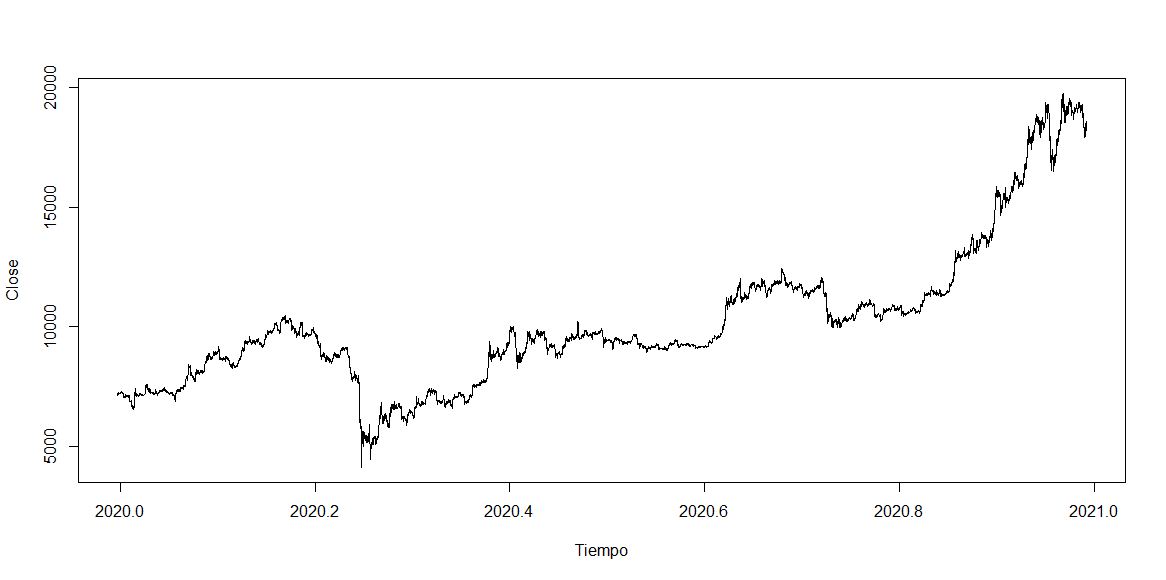
\includegraphics[width=1\textwidth]{serie}
\caption{Serie de tiempo del precio del Cierre del Bitcoin desde el día $12/12/2019$ a las 08:00:00h hasta el $10/12/2020$ a la 01:00:00h.}
\label{priceClose}
\end{figure*}


La base se estructuró de modo de tener un conjunto de entradas $X$ y salidas $Y$ con una dependencia temporal. La variable de predicción $Y$ corresponde al $Cierre$ del precio del Bitcoin en el tiempo $n$. Las entradas correspondientes a $X$ se encuentran en diversos momentos del pasado. 

La variable $Volumen$ corresponde al tiempo $n-1$ ya que es información que no existe a la hora de predecir el momento $n$.

Se crearon variables  de retraso llamadas $lag$, para el precio de $Cierre$ y $Volumen$ de Bitcoin. Los números utilizados para nombrar las variables de retraso, representan el tiempo del pasado. Por ejemplo la variable $closeLag3$ representa el precio del $Cierre$ del Bitcoin 3 horas previas al momento $n$~\cite{forecastinBitcoinClosing}.  

Dada la experiencia previa obtenida a partir de investigaciones y la literatura existente las variables utilizadas son los cinco primeros retrasos del precio del $Close$ y del $Volumen$ del Bitcoin. En la base de datos estas variables son definidas como $closeLag1$, $closeLag2$, $closeLag3$, $closeLag4$, $closeLag5$ $volLag1$, $volLag2$, $volLag3$, $volLag4$ y $volLag5$ respectivamente.

\section{Los modelos}


\subsection{Metodología}

En esta sección presentamos las cuatro técnicas utilizadas que incluyen Modelos Lineales, métodos de ensamble de modelos, Bagging basado en Árboles de decisión y Redes Neuronales.

Un modelo de regresión lineal múltiple (\ref{ecuacionML}) es un modelo lineal en los parámetros en el cual la variable de respuesta, $Y$, es determinada por un conjunto de variables independientes, las variables explicativas (matriz $X$). Se busca el hiperplano que mejor ajuste a los datos. Los parámetros $\beta_i$ para el modelo se obtienen por mínimos cuadrados.

\begin{equation}
y_{i}=\beta_{0}+\beta_{1} x_{i}+\beta_{2} x_{i}+\cdots+\beta_{d} x_{i}+\epsilon_{i}
\label{ecuacionML}
\end{equation}

Los métodos de ensamble de modelos son útiles para mejorar el rendimiento de los modelos de aprendizaje automático al mejorar su precisión. Se construyen varios modelos y se combinan las predicciones resultantes mediante su promedio. Este promedio de errores produce mejores predicciones generalizando el carácter particular de cada uno de estos modelos.

Un árbol de decisión es una división recursiva del espacio de variables explicativas en una estructura en forma de árbol, cada nodo interior contiene una pregunta sobre una variable de entrada y cada nodo terminal una decisión. Estos pueden ser utilizados en problemas de regresión y clasificación, en nuestro caso la variable explicada es continua por lo que trabajamos con árboles de regresión.  

Los árboles CART (Classification And Regression Tree) se construyen dividiendo el conjunto de valores posibles de $X_1,X_2,...,X_p$ en $J$ regiones disjuntas $R_1, R_2,..., R_J$. En el caso de un árbol de regresión, para cada observación en la región $R_j$ se predice el valor medio de las respuestas.

Para llevar a cabo la construcción del árbol se comienza con un conjunto de datos de entrenamiento, el cual es segmentado mediante particiones binarias. Se crean regiones $R_1, R_2,..., R_J$ de manera que se minimice la siguiente ecuación.

$$
\sum_{j=1}^{J} \sum_{i \in R_{j}}\left(y_{i}-\hat{y}_{R_{j}}\right)^{2}
$$

Donde $\hat{y}_{R_{j}}$ es la respuesta media para las observaciones del conjunto de entrenamiento en la región j-ésima~\cite{libroCurso}.

Una vez que se encuentra la mejor partición, se separan los datos en las regiones resultantes y se repite el proceso. Este proceso termina cuando se satisface algún criterio de parada.

El método Bagging (Bootstrap Aggregating) es un procedimiento para reducir la varianza de un modelo de aprendizaje automático~\cite{libroCurso}.

Se divide el conjunto de datos en entrenamiento $L$ y testeo $T$, se toma una muestra bootstrap $L_b$ de $L$ y se construye un estimador usando $L_b$. Se repite el procedimiento $B$ veces. Luego a cada dato de $T$ se le asigna el promedio de las respuestas de los estimadores construidos en el paso anterior (para el caso de un modelo de regresión). La proporción de veces que la clase estimada difiere de la verdadera es el error Bagging. Luego puede repetirse la división de los datos en $L$ y $T$ varias veces y calcular los errores promedio.

Bagging puede ser utilizado para Árboles de decisión, para esto se construyen $B$ árboles con conjunto de entrenamiento obtenido mediante una muestra bootstrap del conjunto de entrenamiento original, luego se hace un promedio de las predicciones resultantes. Estos árboles tienen varianza grande pero sesgo bajo ya que no se podan. Al promediarlos se reduce la varianza y por lo tanto se mejora la precisión de las predicciones.

Las Redes Neuronales son un modelado matemático que homologa el comportamiento de una neurona biológica. El objetivo de su diseño es emular al cerebro humano. Básicamente se basa en una red de neuronas conectadas que reciben un estímulo de entrada y producen una salida.   

En su modelado matemático se construyen combinaciones lineales de las entradas y se obtiene la salida como una función no lineal de estas. 

En la Ecuación (\ref{ecuacionRedes}) se muestra el modelado de una red neuronal con una capa de entrada, una capa oculta y una salida. Donde $i$, $j$ son los índices correspondientes a la capa de entrada y oculta respectivamente, $w$ corresponde a los pesos de cada neurona y $f(.)$ a la función de activación.

\begin{equation}
g_{k}(x)=f \underbrace{(\sum_{j=1}^{n_{H}} w_{k j} f \underbrace{\left(\sum_{i=1}^{d} w_{j i} x_{i}+w_{j 0}\right)}_{\text {net }_{j}}+w_{k 0})}_{\text {net }_{k}}
\label{ecuacionRedes}
\end{equation}

El procedimiento para encontrar los pesos que configuren el mejor modelo consiste en primero multiplicar cada dato de entrada por un peso y los valores ponderados se combinan linealmente. Posteriormente se aplica una función de activación no lineal. El valor de salida es comparado con el valor objetivo. La diferencia de error que se produce es utilizada para actualizar los pesos y se itera hasta obtener el criterio deseado de parada. Actualmente el algoritmo más utilizado para esto es el de Backpropagation. Esta arquitectura crece en complejidad pero el algoritmo y los procesos son siempre los mismos. 

\begin{equation}
(min)RMSE=\sqrt{\frac{1}{N} \sum_{i=1}^{N}\left(y_{i}-f_{i}\right)^{2}}
\label{remseequation}
\end{equation}

Para evaluar el rendimiento de los distintos modelos de predicción se utilizó la medida de error RMSE como se ve en la Ecuación (\ref{remseequation}) donde $y_i$ representa las predicciones y $f_i$ los valores reales. Se busca minimizar el RMSE.

\subsection{Proceso}

En primer lugar, el conjunto de datos se dividió aleatoriamente, en una muestra de entrenamiento del $70\%$ y una muestra de testeo del $30\%$ donde se busca generalizar el comportamiento del precio del Bitcoin en ambas muestras.

El primer objetivo fue recrear la predicción del precio del Bitcoin mediante la estrategía de modelos lineales propuestas en la literatura e investigaciones anteriores. 

En la Figura \ref{diagramLinearRegression} se muestra el diagrama del proceso. En este caso para encontrar el modelo con mejor rendimiento se construyó un algoritmo de fuerza bruta que evalúa secuencialmente una a una todas las posibles combinaciones de las variables seleccionadas (cinco primeros retrasos de $Close$ y $Volumen$ del precio del Bitcoin) comparando el RMSE generado por cada una de estas combinaciones con la muestra de testeo. El modelo seleccionado es aquel con el menor RMSE. El orden de todas las combinaciones es de $2^n - 1$ para $n$ opciones de variables. En este caso contamos con $1023$ posibles modelos.


\begin{figure}[!hbt]
\centering
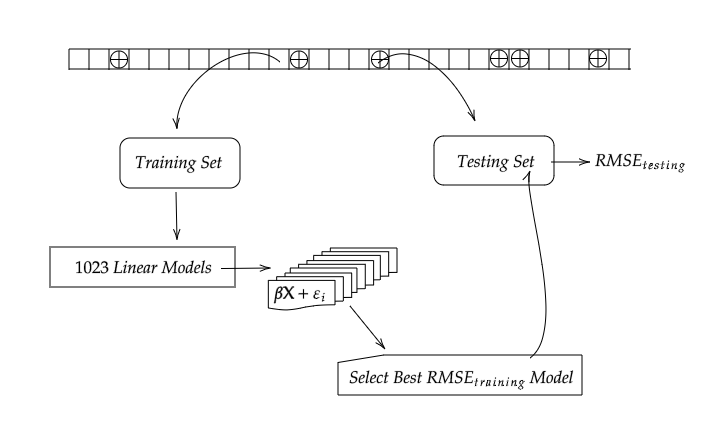
\includegraphics[width=0.5\textwidth]{diagramLinearRegression}
\caption{Diagrama del proceso de generación del modelo lineal con menor RMSE a partir de una selección de $1023$ posibles modelos creados desde las combinaciones obtenidas de los cinco primeros retrasos de $Close$ y $Volumen$ del precio del Bitcoin.}
\label{diagramLinearRegression}
\end{figure}

En la búsqueda de nuevas propuestas de predicción, mediante la prueba y el error y otras sugerencias de la literatura existente, decidimos primariamente cambiar el enfoque de generación de muestras de entrenamiento y testeo estáticas hacia un enfoque dinámico mediante el concepto de ventanas móviles \cite{forecastinBitcoinClosing}. 

El concepto de ventanas móviles consiste en que para predecir el precio del Bitcoin del momento $n$ se genera una ventana de entrenamiento con memoria de corto plazo de un ancho de $w$ rezagos de tiempo. Es decir, una ventana de $w$ rezagos para la predicción del momento $n$ iría desde el momento $n-1$ hasta el momento $n-w-1$. En esta investigación se utiliza una ventana móvil de 25 rezagos, esto es producto de diferentes pruebas y recomendaciones en la literatura. 

El siguiente paso fue utilizar el concepto previamente descripto para modelos lineales pero en las ventanas móviles de corto plazo. Es decir, que para cada momento $n$ que se quiere predecir se generan $1023$ modelos lineales a partir de todas las combinaciones de las variables. En este punto surgieron descubrimientos importantes que dirigieron el rumbo de esta invesigación. 

Una primer conclusión fue notar que la linealidad en cada una de las ventanas móviles era extremadamente fuerte ya que el RMSE obtenido con las mismas muestras de entrenamiento de cada ventana era considerablemente bajo y a medida que aumentabamos el $w$ de la ventana el RMSE aumentaba. Esto fue un indicio de que utilizar modelo lineales era una buena opción ya que la linealidad en el corto plazo era fuerte.

Otro punto importante para el desarrollo de esta investigación fue el descubrimiento de que entre las $1023$ predicciones obtenidas por los modelos lineales en cada ventana en un  $76.15\%$ de los casos al menos uno de los modelos realizaba una estimación casi perfecta en un intervalo $\pm 5$ dólares. 

En la Figura \ref{muestras} se puede observar como en una muestra aleatoria de cuatro momentos de la base, en las primeras tres muestras el precio de $Close$ es contemplado en al menos una de las $1023$ predicciones. En la muestra $4$ se observa como ninguna de estas estimaciones logra predecir con una exactitud de $\pm 5$ dólares este precio. Este comportamiento se mantiene durante toda la base.

\begin{figure}[!htb]
\centering
\subfigure[Muestra 1.]
{ 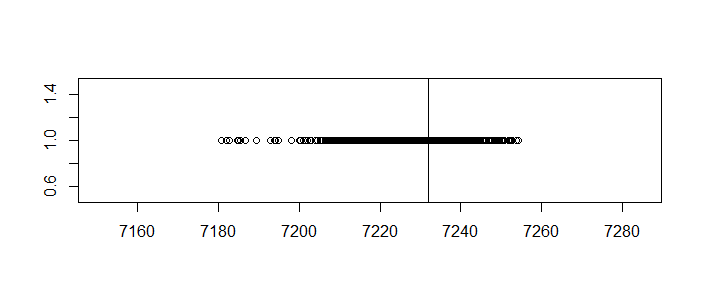
\includegraphics[width=5.0cm]{muestra1}
\label{pca_MORT}
}\\
\subfigure[Muestra 2.]
{ 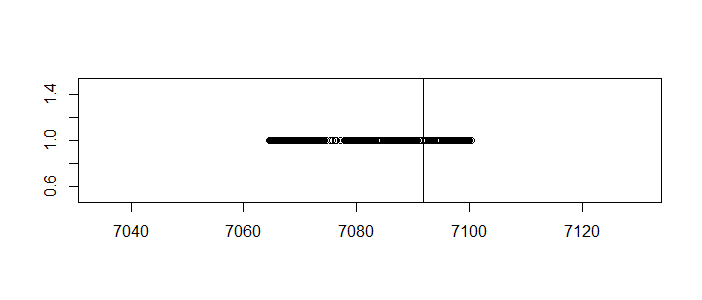
\includegraphics[width=5.0cm]{muestra2}
\label{pca_HUMID}
}\hfill
\subfigure[Muestra 3.]
{ 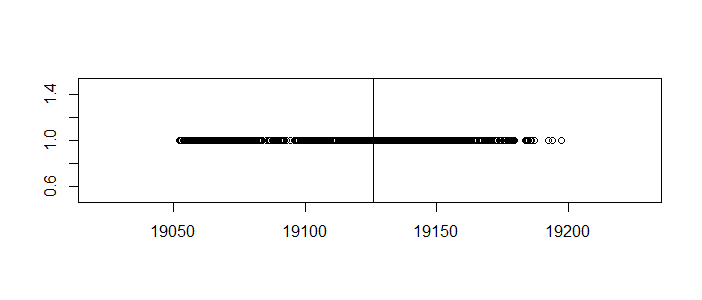
\includegraphics[width=5.0cm]{muestra3}
\label{pca_NOX}
}\hfill
\subfigure[Muestra 4.]
{ 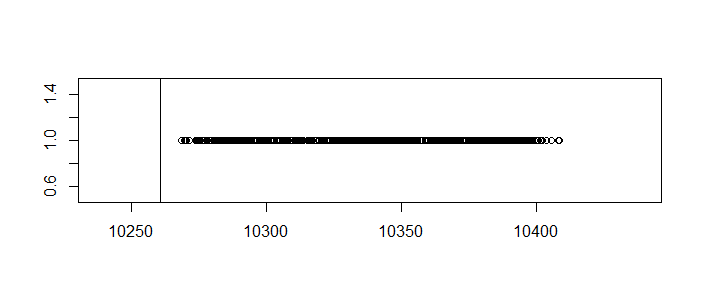
\includegraphics[width=5.0cm]{muestra4}
\label{pca_HOUS}
}
\caption{Muestra de cuatro momentos de la base y las $1023$ predicciones del precio de $Close$ generadas a partir de una ventana de $25$ rezagos para cada momento por modelos lineales.}
\label{muestras}
\end{figure}
%

De aquí en adelante en esta investigación la estrategía a seguir es la de buscar posibles patrones entre los precios estimados por cada uno de los modelos y el precio real de $Close$ del Bitcoin. Por los ejemplo simplificando, ¿existe una relación cada vez que los primeros diez modelos predicen un precio muy cercano en sus predicciones y el precio real del $Close$? Los posibles patrones a encontrar entre estas posibles predicciones y el precio real son muchos, entonces nuestra pregunta fundamental a responder es ¿existe algún patrón entre las $1023$ predicciones y el precio real del Bitcoin?

\begin{figure}[!hbt]
\centering
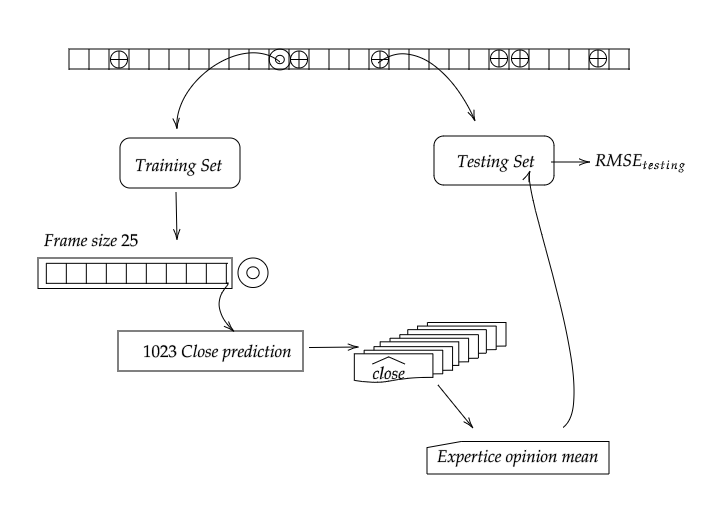
\includegraphics[width=0.5\textwidth]{diagramExpertMean}
\caption{Diagrama.}
\label{diagramLinearRegression}
\end{figure}

\begin{figure}[!hbt]
\centering
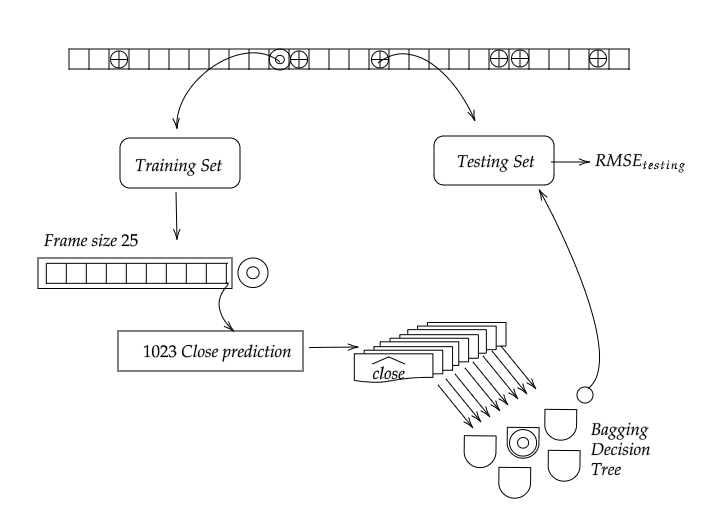
\includegraphics[width=0.5\textwidth]{diagramBagging}
\caption{Diagrama.}
\label{diagramLinearRegression}
\end{figure}

\begin{figure}[!hbt]
\centering
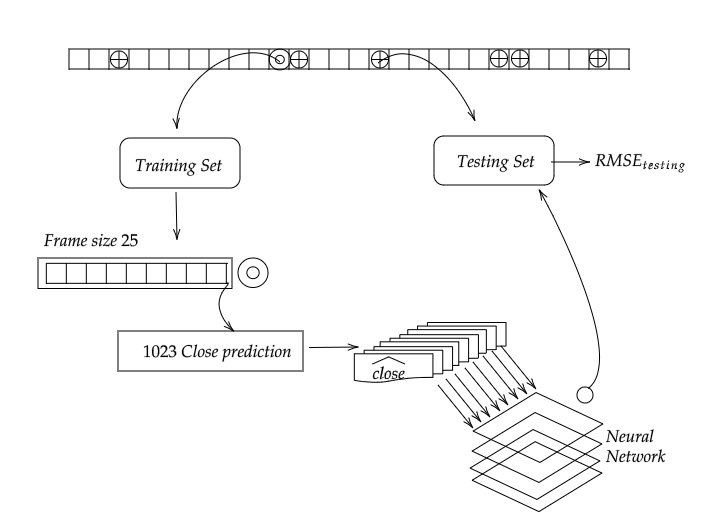
\includegraphics[width=0.5\textwidth]{diagramNeuralNetwork}
\caption{Diagrama.}
\label{diagramLinearRegression}
\end{figure}



\section{Resultados}

El objetivo de  esta investigación es evaluar la predicción del precio de $Cierre$ del Bitcoin mediante algoritmos de Aprendizaje automático. 

En primer lugar, para el caso de Árboles de regresión y Bagging se buscó encontrar el modelo con menor RMSE mediante un algoritmo de fuerza bruta. Este algoritmo evalúa todos los posibles modelos generados a partir de todas las combinaciones posibles de 12 variables seleccionadas mediante prueba y error. Estas variables son $trend$ (las tendencias de búsqueda en Google), $ltcOpen$ (precio de $Apertura$ de Litecoin), $closeLag1$, $closeLag2$, $closeLag3$, $closeLag4$, $closeLag5$ (cinco primeros retrasos del precio de $Cierre$ de Bitcoin), $volLag1$, $volLag2$, $volLag3$, $volLag4$, $volLag5$ (cinco primeros retrasos del $Volumen$ de Bitcoin). Para estas técnicas se utilizó el paquete randomForest~\cite{randomForest} de R~\cite{r}.

En la Figura ~\ref{decisionTree}  se muestra el Árbol de regresión con menor RMSE obtenido para predecir el precio de Cierre del Bitcoin basado en el retraso del Cierre de un día. La división en la parte superior del árbol da como resultado dos ramas grandes. A modo de ejemplo, la rama de la izquierda corresponde a $closeLag1<8182$, lo que representa al $22\%$ de las observaciones, y la rama de la derecha corresponde a $closeLag1 \geq 8182$, el $78\%$ de las observaciones. La rama izquierda se vuelve a dividir. La nueva rama izquierda representa las observaciones que tienen un $closeLag1<6415$, el $7\%$ de ese $22\%$ inicial; y la rama derecha representa las observaciones que tienen un  $closeLag1 \geq 6415$ y además un $closeLag1<8182$, estas son el $15\%$ restante de las observaciones. Estos últimos dos nodos son llamados terminales u hojas y el número en cada una de estas es la media de la respuesta de las observaciones que se encuentran allí. Este árbol tiene cuatro nodos internos y cinco nodos terminales u hojas.

Es importante recalcar que de los $4095$ ($2^{12} - 1$) posibles modelos resultantes por el algoritmo de fuerza bruta, $2048$ modelos obtienen el menor RMSE de $537.6748$. En este caso por el principio de parsimonia se selecciona el modelo con menor cantidad de variables, el cual sólo consta de una variable que es el primer retraso del precio de $Cierre$ del Bitcoin. 
Esto es un punto interesante, ya que como se menciona en~\cite{forecastinBitcoinClosing}, esto confirma la hipótesis que la serie del precio del Bitcoin en su medida histórica global es indistinguible de un paseo aleatorio. 

\begin{figure}[!hbt]
\centering
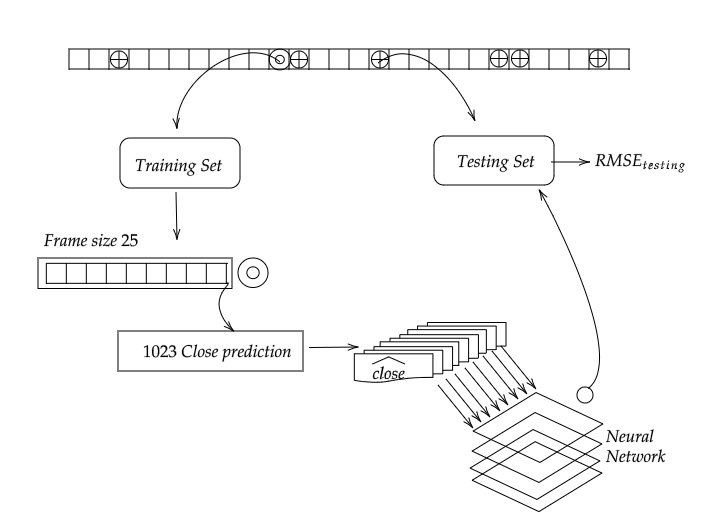
\includegraphics[width=0.5\textwidth]{diagramNeuralNetwork}
\caption{Árbol de regresión correspondiente al precio de Cierre del Bitcoin.}
\label{decisionTree}
\end{figure}

En el caso de Bagging el modelo que logra un menor RMSE de $454.5812$ está compuesto por las variables $trend$, $closeLag1$, $closeLag2$, $closeLag3$, $volLag3$, $volLag5$ y $ltcOpen$. En el Cuadro~\ref{baggingTop10} se muestran los diez modelos que lograron el menor RMSE con esta técnica. En la Figura~\ref{baggingVariableImportancia}  se muestra la media de precisión en las predicciones en la muestra cuando cada una de las variables se excluye del modelo. Es interesante como se destaca la importancia de la variable $closeLag1$ con respecto a las demás variables que forman el modelo, siendo esto concluyente con la hipótesis previamente mencionada de que el precio del Bitcoin es un camino aleatorio. 


\begin{figure*}[!hbt]
\centering
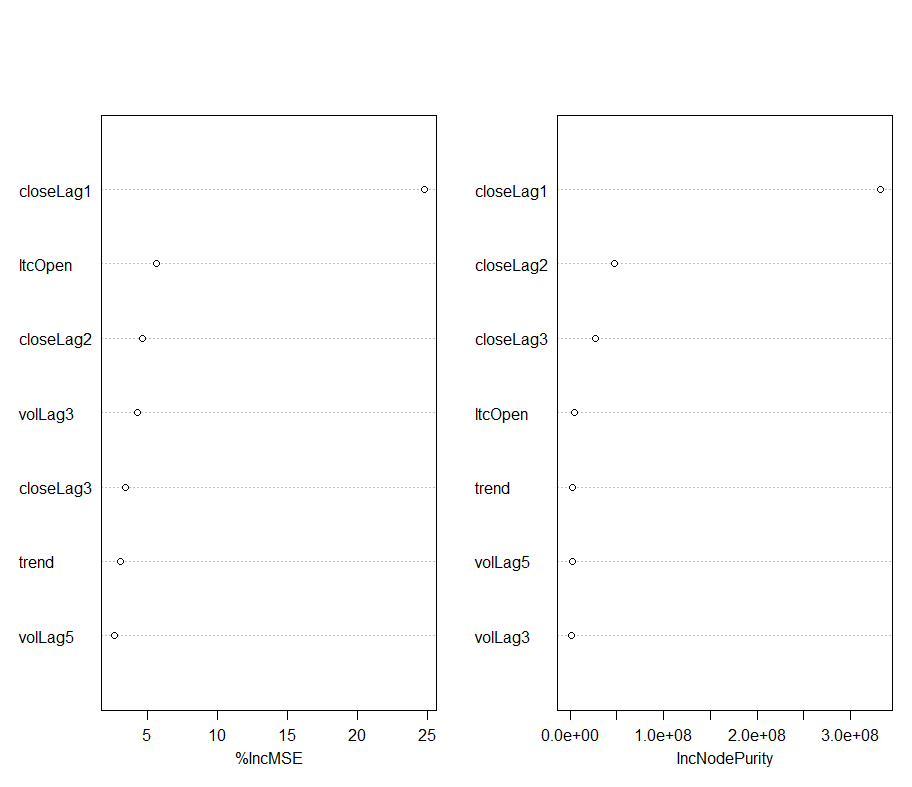
\includegraphics[width=0.7\textwidth]{baggingVariableImportancia}
\caption{A la izquierda se muestra la disminución media de la precisión en las predicciones en la muestra OOB cuando una variable determinada se excluye del modelo (IncMSE). A la derecha se muestra la disminución total en la impureza del nodo que resulta de las divisiones sobre esa variable, promediada en todos los árboles para regresión (IncNodePurity).}
\label{baggingVariableImportancia}
\end{figure*}

Otro indicador de error de prueba es el error out-of-bag (OOB). Los árboles que se construyen en Bagging se generan con muestras bootstrap que utilizan aproximadamente dos tercios de las observaciones originales, las restantes son llamadas out-of-bag. Para el caso de regresión se puede calcular el RMSE OOB, este sirve como una estimación del error de prueba debido a que la respuesta para cada observación se predice utilizando solamente los árboles que no se ajustaron con dicha observación. Este es incluso una aproximación al error de validación cruzada dejando uno fuera cuando el número de árboles es suficientemente grande, en nuestro caso el número de árboles empleados es de 100. Aplicando el RMSE OOB en el modelo final de Bagging se obtiene un resultado de $467.7928$. Esto nos da a entender que el modelo en otras circunstancias de predicción sigue teniendo un comportamiento similar ya que la diferencia con el RMSE es baja.

\begin{table*}[!hbt]
\centering
\caption{Variables utilizadas para los mejores 10 modelos y su RMSE correspondiente para la predicción del precio de $Cierre$ de Bitcoin utilizando Bagging.}
\label{baggingTop10}
\begingroup\setlength{\fboxsep}{0pt}
\colorbox{lightgray}{%
\begin{tabular}{|l|l|}
\hline Modelo & RMSE \\
\hline  trend, closeLag1, closeLag2, closeLag3, volLag3, volLag5, ltcOpen & 454.5812\\
\hline trend, closeLag1, closeLag3, volLag2, volLag3, volLag4, volLag5, ltcOpen & 456.4094 \\
\hline   trend, closeLag1, closeLag3, closeLag4, closeLag5, volLag1, volLag3, \\volLag4, volLag5, ltcOpen& 459.2152 \\
\hline  trend, closeLag1, closeLag2, closeLag4, volLag3, volLag4, volLag5& 459.6356 \\
\hline  trend, closeLag1, closeLag2, closeLag3, closeLag4, volLag3, volLag5& 459.7546\\
\hline trend, closeLag1, closeLag2, closeLag3, volLag2, volLag3, volLag5, \\ ltcOpen & 459.7760\\
\hline trend, closeLag1, closeLag3, volLag1, volLag3, volLag4, volLag5, \\ ltcOpen & 460.0010\\
\hline trend, closeLag1, closeLag2, closeLag4, volLag3, volLag5, ltcOpen & 460.0387\\
\hline trend, closeLag1, closeLag3, closeLag4, volLag1, volLag2, volLag3, \\ volLag4, volLag5, ltcOpen & 460.5488\\
\hline trend, closeLag1, closeLag3, closeLag5, volLag1, volLag2, volLag3, \\ volLag4, volLag5, ltcOpen & 460.6552\\
\hline
\end{tabular}%
}\endgroup
\end{table*}

Para las Redes Neuronales se utilizó el paquete Keras~\cite{keras} de R~\cite{r} que es una capa de alto nivel de Tensorflow~\cite{tensorflow}. Tensorflow es una biblioteca de código abierto propiedad de Google y de las más utilizadas actualmente para el aprendizaje profundo. En el Cuadro~\ref{redesModelTuning} se muestran los RSME obtenidos por distintas configuraciones de capas y funciones de activación. En particular para todas las redes se utilizaron las mismas variables de entrada  las cuales son las obtenidas por el modelo con menor RMSE de Bagging ($trend$, $closeLag1$ , $closeLag2$ , $closeLag3$ ,  $volLag3$ , $volLag5$ y $ltcOpen$). Todas las redes constaban de 3 capas ocultas, donde la primera capa oculta es utilizada para la estandarización de los valores de las variables de entrada. La segunda capa oculta se probó con 8 y 16 nodos y funciones de activación linear y relu. La  tercer capa se probó con 8 nodos y funciones relu. La tendencia de los nodos y capas probados mostraron que al agregar más nodos en las capas se obtenían mejores resultados. Estos algoritmos emplean una gran cantidad de procesos informáticos, por lo que probar con más nodos y capas, exigía un poder computacional fuera del alcance técnico empleado para esta investigación. 


\begin{table*}[!hbt]
\centering
\caption{Combinaciones de banderas utilizadas en las Redes Neuronales y el RMSE obtenido para la predicción del $Cierre$ de Bitcoin. }
\label{redesModelTuning}
\begingroup\setlength{\fboxsep}{0pt}
\colorbox{lightgray}{%
\begin{tabular}{|l|l|l|l|l|}
\hline Capa de nodos 2 & Capa de nodos 3 & Capa de activación 2 & Capa de activación 3 & RMSE \\
\hline 16 & 8 & relu & relu  &  136.8908\\
\hline 8 & 8 & relu & relu  &  10640.92\\
\hline
\end{tabular}%
}\endgroup
\end{table*}

En el Cuadro~\ref{RMSEFinal} se muestra el desempeño de cada uno de los modelos seleccionados por las técnicas empleadas (Bagging, Árboles de decisión y Redes Neuronales). En este caso el modelo seleccionado para Bagging es el que logra mejores resultados. A la vez la tabla muestra, como la flexibilización del algoritmo, no necesariamente arroja mejores resultados. También en nuestra investigación anterior~\cite{paper1}, donde se utilizaron algoritmos de Aprendizaje Automático menos flexibles, los RMSE obtenidos son ampliamente menores que los de esta investigación. En particular con Modelos Lineales se logra un RMSE de $291.971$.

En el caso de Modelos Lineales las variables que se obtuvieron en el modelo fueron $trend$, $closeLag1$, $closeLag2$, $closeLag4$,  $volLag1$, $volLag3$, $volLag4$ y $ltcOpen$. Es interesante notar que solo existen diferencias de los valores de retrasos pero las variables son las mismas que en el modelo obtenido por Bagging en esta investigación. 

\begin{table}[!hbt]
\centering
\caption{Mejores resultados de RMSE obtenidos para las cuatro técnicas utilizadas en la predicción del $Cierre$ de Bitcoin. }
\label{RMSEFinal}
\begingroup\setlength{\fboxsep}{0pt}
\colorbox{lightgray}{%
\begin{tabular}{|l|l|}
\hline Algoritmo de predicción & RMSE \\
\hline Modelos Lineales & 231.4537\\
\hline Ensamble de modelos & 91.33031\\
\hline Bagging (Árbol de decisión)& 78.87432\\
\hline Redes Neuronales & 136.8908 \\
\hline
\end{tabular}%
}\endgroup
\end{table}
   
\section{Conclusiones}

Los resultados obtenidos muestran que entre los métodos utilizados en esta investigación, la técnica de Bagging es la que obtiene mejores resultados para la predicción del precio de $Cierre$ del Bitcoin. Sin embargo, estos métodos más flexibles no obtuvieron mejores resultados que estudios previos con modelos menos flexibles, en particular Modelo Lineales. 

A futuro se plantea la posibilidad de utilizar Bagging para estabilizar los modelos obtenidos de Redes Neuronales. También se mostró una tendencia a la mejora del desempeño en cuanto se aumentaba la cantidad de nodos y conexiones en las Redes Neuronales, por lo que probar modelos con más capas, nodos y conexiones complejas, es una opción a investigar en próximas instancias.
     

\newpage  
\onecolumn              
%
\begin{thebibliography}{99}

\bibitem{Bitcoin_revolucion_monetaria}
Sangoi, F.
{\em Bitcoin. ¿Una revolución monetaria?}
Universidad de Buenos Aires.
%
\bibitem{regression_for_bitcoin_price}
Azim Muhammad Fahmi, Noor Azah Samsudin, Aida Mustapha, 
Nazim Razali, Shamsul Kamal Ahmad Khalid. (2018).
{\em Regression based Analysis for Bitcoin Price Prediction.}
Faculty of Computer Science and Information Technology, Universiti Tun Hussein Onn Malaysia.

\bibitem{Satoshi}
Nakamoto, S. (2008).
{\em Bitcoin: A Peer-to-Peer Electronic Cash System.}

\bibitem{Blockchain}
Carlos Dolader Retmal et al.
{\em La blockchain: fundamentos, aplicaciones y relación con otras tecnologías disruptivas}, Universitat Politécnica de Catalunya.

\bibitem{Blockchain_science}
Karame, G., Huth, M., Vishik, C. (2020).
{\em An overview of blockchain science and
engineering.} R. Soc. Open Sci. 7: 200168.
http://dx.doi.org/10.1098/rsos.200168


\bibitem{Bayesian}
Shah, D., Zhang, K. (2014).
{\em Bayesian regression and Bitcoin.} 
Laboratory for Information and Decision Systems
Department of EECS, Massachusetts Institute of Technology.


\bibitem{Methods}
Ferdiansyah, Siti Hajar Othmanb, Raja Zahilah Raja Md Radzic, Deris Stiawan. (2019).
{\em A Study of Bitcoin Stock Market Prediction: Methods, Techniques and Tools.} 

\bibitem{Bitcoin_bubbles_predictable}
Wheatley, S., Sornette, D., Huber, T., Reppen, M., Gantner, RN. (2019). 
{\em Are Bitcoin bubbles predictable? Combining a generalized
Metcalfe’s Law and the Log-Periodic Power Law
Singularity model.} R. Soc. open sci. 6: 180538.
http://dx.doi.org/10.1098/rsos.180538

\bibitem{forecastinBitcoinClosing}
Uras, N., Marchesi, L., Marchesi, M., Tonelli, R. (2020)
{\em Forecasting Bitcoin closing price series using linear
regression and neural networks models}. Department of Mathematics and Computer Science, University of Cagliari.

\bibitem{forecast_bitcoin_GAM}
Asante Gyamerah, S. (2020).
{\em On forecasting the intraday Bitcoin price using ensemble of variational
mode decomposition and generalized additive model}. Pan African University, Institute for Basic Sciences, Technology, and Innovation.
https://doi.org/10.1016/
j.jksuci.2020.01.006


\bibitem{bitcoin_ML}
McNally, S. (2016).
{\em Predicting the price of Bitcoin using Machine Learning.} School of Computing National College of Ireland.

\bibitem{mainDriversBitcoin}
Kristoufek, L. (2015). {\em What Are the Main
Drivers of the Bitcoin Price? Evidence from Wavelet
Coherence Analysis.} PLoS ONE 10(4): e0123923.
doi:10.1371/journal.pone.0123923

\bibitem{bitcoin_ML_PSA}
Rajua, S., Mohammad, A. (2020).
{\em Real-Time Prediction of BITCOIN Price using Machine Learning Techniques and Public Sentiment Analysis.}
Computer Science, International Islamic University Malaysia.

\bibitem{bitcoin_socialmedia}
Burnie, A., Yilmaz, E. (2019). 
{\em Social media and bitcoin metrics: which words matter.}
R. Soc. open sci. 6: 191068.
http://dx.doi.org/10.1098/rsos.191068

\bibitem{bitcoin_socialmedia}
Garcia, D., Schweitzer, F. (2015).
{\em Social signals and algorithmic trading of Bitcoin.} R. Soc. open sci. 2: 150288.
http://dx.doi.org/10.1098/rsos.150288

\bibitem{Predictor_Impact_Web_Search_Media__Bitcoin_Trading_Volumes}
Matta, M.; Lunesu, I. and Marchesi, M.  (2015).
{\em The Predictor Impact of Web Search Media On Bitcoin Trading Volumes.}
Universita’ degli Studi di Cagliari.

\bibitem{Bitcoin_variables}
Hakim, R. (2020)
{\em Bitcoin pricing: impact of attractiveness variables.}
Sao Paulo School Of Economics.
https://doi.org/10.1186/s40854-020-00176-3

\bibitem{r}
R Core Team. (2020). 
{\em R: A Language and Environment for Statistical Computing.}
Vienna, Austria: R Foundation for Statistical Computing. 
https://www.R-project.org/

\bibitem{tree}
Ripley, B. (2019). 
{\em tree: Classification and Regression Trees.}
https://CRAN.R-project.org/package=tree

\bibitem{randomForest}
Liaw, A., Wiener, M. (2002). 
{\em Classification and Regression by randomForest.}
https://CRAN.R-project.org/doc/Rnews/

\bibitem{keras}
Allaire, JJ., Chollet, F. (2020).
{\em keras: R Interface to 'Keras'.}
https://CRAN.R-project.org/package=keras

\bibitem{tfdatasets}
Allaire, JJ., Tang, Y., Ushey, K. (2020).
{\em tfdatasets: Interface to 'TensorFlow' Datasets.}
https://CRAN.R-project.org/package=tfdatasets

\bibitem{tfruns}
Allaire, JJ. (2018).
{\em tfruns: Training Run Tools for 'TensorFlow'.}
https://CRAN.R-project.org/package=tfruns

\bibitem{tensorflow}
Allaire, JJ., Tang, Y. (2020).
{\em tensorflow: R Interface to 'TensorFlow'.}
https://CRAN.R-project.org/package=tensorflow

\bibitem{libroCurso}
Gareth, J., Witten, D., Hastie, T., Tibshirani, R. (2013). 
{\em An introduction to statistical learning : with applications in R.}
New York: Springer.

\bibitem{libroCurso2}
Hastie, T., Tibshirani, R., Friedman, J. (2017). 
{\em The Elements of Statistical Learning: Data Mining, Inference, and Prediction.}
New York: Springer, 2nd edition.

\bibitem{paper1}
Alcalde, V., Martinez Angerosa, P. (2020). 
{\em Predicción del precio diario de Cierre y dirección del Bitcoin mediante Modelos de Regresión Lineal Múltiple y Logísticos.}

\bibitem{paper2}
Alcalde, V., Martinez Angerosa, P. (2020). 
{\em Predicción del precio diario de Cierre del
Bitcoin mediante Bagging, Árboles de
decisión y Redes Neuronales.}

\bibitem{Goodfellow}
Goodfellow, I., Bengio, Y., Courville, A. (2016). 
{\em Deep Learning.} MIT Press. 
http://www.deeplearningbook.org


\end{thebibliography}
\end{document}
